%%%%%%%%%%%%%%%%%%%%%%%%%%% START WITH LATEX PREAMBLE %%%%%%%%%%%%%%%%%%%%%%
% reminder: its = possessive
%           it's = it + is

%use [11pt, draft] for draft markings.
\documentclass[11pt]{mvlthesis}
\usepackage[dvipdfmx]{graphicx}
\usepackage{verbatim} %,amssymb,amsmath}
\usepackage{pdfpages}
% load package with some of the available options - you may not need this!
\usepackage[framed,autolinebreaks,useliterate]{mcode}
%\usepackage{afterpage}
\usepackage{url}

%%%%%%%%%%%%%%%%%%%%% SET UP ALL THE TITLE PAGE VARIABLES %%%%%%%%%%%%%%%%%%

\title{\scshape \mbox{Simplex Control and Message/ACK Exchange}\\
\scshape \mbox{ECE4305 Final Project Module 6}}

\author{Renato Iida, Le Wang, Rebecca Copper}


\thesis_or_diss{Project Report}
\degree_type{ECE 4305}
\field{Electrical and Computer Engineering Department}

%\degreeyear{MONTH YEAR}
%\chair{Professor X}
%\chairtitle{Major Advisor}
%\membertwo{Professor Y}
%\memberthree{Professor Z}


%%%%%%%%%%%%%%%%%%%%%% INCLUDE USER DEFINED COMMANDS %%%%%%%%%%%%%%%%%%%%%%%

\newcommand{\bi}{\begin{itemize}}
\newcommand{\ei}{\end{itemize}}
\newcommand{\ii}{\item}
\newcommand{\be}{\begin{enumerate}}
\newcommand{\ee}{\end{enumerate}}
\newcommand{\ie}{\item}

\newcommand{\fig}[5]{
    \begin{figure}[#1]
    \begin{center}
    \includegraphics[#2]{#3}
    \end{center}
    \caption{#4}
    \label{#5}
    \end{figure}
}

%\frenchspacing

%%%%%%%%%%%%%% SPECIFY WHICH PARTS OF THE THESIS YOU WANT PRINTED %%%%%%%%%%

\renewcommand{\baselinestretch}{1.5}

\newcommand{\pderiv}[2]{\mbox{$\frac{\displaystyle \partial #1}{\displaystyle \partial #2}$}}

%%%%%%%%%%%%%%%%%%%% Done with setup, document starts here %%%%%%%%%%%%%%%%%
\begin{document}


%%%%%%%%%%%%%%%%%%%%%%%%%%%%%% TITLE + ABSTRACT %%%%%%%%%%%%%%%%%%%%%%%%%%%%
\maketitle
\begin{abstract}

Put your abstract here.

\end{abstract}

%%%%%%%%%%%%%%%%%%%%%% ACKNOWLEDGMENTS + TABLE OF CONTENTS %%%%%%%%%%%%%%%%%

\begin{frontmatter}


\tableofcontents
\listoffigures
\listoftables

\end{frontmatter}

%%%%%%%%%%%%%%%%%%%% INCLUDE THE REST OF THE DOCUMENT %%%%%%%%%%%%%%%%%%%%%%


\chapter{Introduction}
\label{ch:introduction}


In Software Defined Radio Systems and Analysis we are using USRPs to create a Cellular Network through Simulink and Matlab. This network is small, made up of only three users (UE1, UE2, and UE3) connected to two base stations (BS1 and BS2). Two users,  UE1 and UE2 are associated with BS1; BS2 only has one client, UE3. Communication in this network will be through time divided channels for each device in the 0.9e9 chunk of the spectrum at FREQUENCYOFNETWORK. Each Base Station will have a dedicated time slot for either intracellular or intercellular communication. The users within each cell will have a time slot as well, though across cells these time slots will intersect. There will be three different standards used to communicate between devices. UE1 will use Standard 1, and UE2 and UE3 will use Standard 2. Each base station will be able to communicate with it's associated user(s) as well as using the higher power Standard 3 to communicate with each other.

This cellular network will send text messages between UEs. These messages must be transferred to the intended receivers through the base stations. To ensure that the message will able to be routed properly through the network and read by the receiver there must be a system of encoding these text messages. This encoding  must be readable by each UE and have the means for each base station to determine the intended receiver. There should also be methods to ensure that the correct message has been received. Team 6 proposed the creation of a MAC frame format that could be sent and decoded by each of the standards and the use of an ACK control packet that could be sent after a properly received message to signal transmission. We will be explaining our final  design as well as the methodology for testing our designs and the results of those tests. 

%pretty sure this could use a better ending, we shall see


% FROM THE PROPOSAL:
%In SDRSaA we are creating a Cellular Network with USRPs using Matlab. This network will be small, made up of only three users (UE 1, UE 2, and UE 3) connected to two base stations (BS 1 and BS 2). There will be three different standards used to communicate between nodes. As shown in Figure 1, UE 1 and UE 2 are associated with BS 1 and BS 1 connects to BS 2. BS 2 only has one client, UE 3. We are assuming all the communications between these nodes are on different channels. UE 1 talks to BS 1 through channel 1, UE2 talks to BS1 on channel 2. There will be at least 4 channels for the system. The USRPs run with Matlab cannot handle full duplex mode so each segment of communication will be in simplex mode. We are also assuming that the network will be static; none of the users will change base stations.
%As Team 6 we will be establishing end-to-end network resource allocation management as well as exchanging of control information and message/ACK forwarding between the UEs and the BS units. Other teams will be creating the three standards and the channels used to transmit messages as well as initializing the network and allocating the resources of each of the base stations.


\chapter{Final prototype design}
\label{ch:design}
This chapter describes the evolution of frame format proposed in \ref{ch:proposal}. Also, it describes the reason for each change based on better understanding the needs of the other teams and the problems in the development. Figure \ref{Interface} is a diagram of our interaction with the other teams that make up this network. 
\begin{figure}[ht]
    \centering
    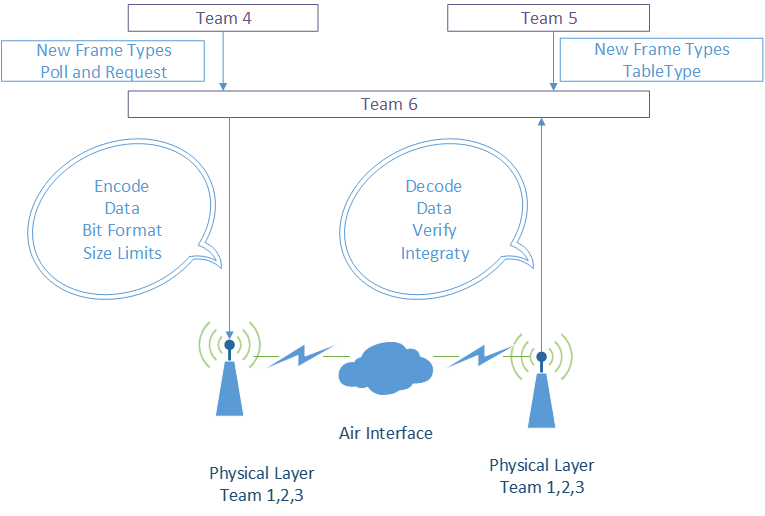
\includegraphics[width=0.8\textwidth]{Interface_diagram.PNG}
    \caption{Diagram of how Module 6 interfaces with the rest of the network}
    \label{fig:Interface}
\end{figure}


\section{MAC Frame Construction}
The structure of a frame is affected by many factors. In this project, in order to make the design as simple as possible, we put the simplicity as the primary factor. That is when there is a conflict between the simplicity and efficiency or other factors, we choose the simplicity, the efficiency or there factors is less important. This section will introduce all the sections of the frame structure one by one in details. 

\subsection{The Services Provided by MAC Layer}

The basic service of our MAC layer is to move a frame from end to end. Basically saying, the MAC layer is implemented below the application layer and above the physical layer. The application layer generates the data and passes it below to the MAC layer. The MAC layer encapsulates the data with a header and a checksum tailer, then pass it to the USRP N210, which is the physical layer. Possible services that can be offered by our MAC layer include: 

\subsubsection{Framing} The MAC layer encapsulates data received from up layers within a MAC frame before transmission to the physical layer. A frame consists of a data field, in which the the data is inserted, and a number of header fields. 
\subsubsection{Reliable delivery} For end-to-end links that have a single sender at one end of the link and a single receiver at the other end of the link, the MAC protocol is simple. When a MAC protocol provides reliable delivery service, it guarantees to move each data across the link without error.  The reliable delivery service can be achieved with acknowledgments and retransmissions. In other words, the MAC layer focuses an end-to-end retransmission if the data is corrupted. 
\subsubsection{Error detection} The receiver can incorrectly decide that a bit in a frame is zero when it was transmitted as a one, and vice versa. Such bit errors are introduced by signal attenuation and electromagnetic noise. The MAC layer protocol provide a mechanism to detect such bit errors, which is done by having the transmitter include error-detection bits in the frame, and having the receiver perform an error check. In this project, we adopted CRC-8 to perform the error detection. 
\subsubsection{Routing Protocols} As the cellular network in the project has no network layer, the MAC layer has to deal with the end-to-end routing protocols. During the process, many protocols have been considered. More details are provided below. 




\subsection{Error-Detection Techniques}
During the communication, it is important to detect the corruption of bits in a MAC frame sent from one node to another node. At the sender, to be protected against bit errors is augmented with error-detection bits, CRC-8 in the project. Typically, the frame to be protected includes not only the data passed down from the application for transmission, but also MAC layer header information. Both data and CRC-8 are sent to the receiver in a MAC frame. At the receiver, a sequence of bits, data and CRC-8 is received. If the CRC-8 differ from the original CRC-8 at the sender, this means there are bit flips in transit.  In this project, we adopted CRC-8 (Cyclic Redundancy Checks-8bits). 

\subsubsection{Cyclic Redundancy Check (CRC-8)}

CRC-8, also known as polynomial codes, is used widely in today's communication networks. For CRC-8, it is possible to view the bit string to be sent as a polynomial whose coefficients are the 0 and 1 values in the bit string, with operations on the bit string interpreted as polynomial arithmetic. The algorithm of CRC-8 is beyond the limit of this report, we use CRC check library of MATLAB directly. 

Before sending the frames, the sender performed CRC check to the header and data respectively and attached the result in the frame. When the receiver received the frame, it performed CRC check again and compare the results with the original CRC results. If the results are the same, which means both the header and the receiver are intact. Otherwise, if the results are different, this means the frame has been corrupted during the transmission. The receiver will drop the corrupted frames. When the timer of the transmitter timeout, the transmitter will send the same frame again to the receiver. 

In order to implement the CRC function, we add 1 byte CRC-8 checksum at the end of the header and another CRC-8 checksum at the end of the data. According to the requirement of the CRC check library in MATLAB, we have to append the CRC checksum at the end of each corresponding section. 



\subsection{Proposals of MAC Frame Types based on Different Routing Protocols}

Basically, the frame should contains at least the sender ID and the receiver ID in order to implement the routing protocols. However, as for the wireless communication, the routing protocol becomes more difficult than wired communication networks. There are several wireless routing protocols in today's network, we will discuss each of them one by one. 

\subsubsection{Ad-hoc based routing protocols}
First, we consider to borrow the idea of the ad-hoc routing protocols. For ad-hoc mode, the frame contains four addresses in the header. So in our MAC frame, there are four addresses too. In addition to the Sender UE ID, Receiver UE ID, we add Sender BS ID, and Receiver BS ID. The sender will send the frame based on the information of Sender ID and Receiver ID, and the base station forwards the frames based on the information of Sender/Receiver BS ID. The disadvantages of this protocol is obvious. First, the frame is very long due to the existence of four IDs, which go against the simplicity requirement. Second, using four addresses may induce redundant information to the transmission. Take a user sender UE for example, when the UE wants to transmit frames, all it needs is the Sender UE ID and the destination UE ID, the information of Sender BS ID and Receiver ID is unnecessary. Based on the above consideration, we did not adopt the this pan.


\subsubsection{Infrastructure based Wi-Fi routing protocols}

The second mechanism we have considered is the routing idea of infrastructure Wi-Fi. The infrastructure Wi-Fi uses three addresses in the frame header. So in our MAC frame header, there are three addresses. In addition to the Sender UE ID and the Receiver UE ID, we add Next Stage section to the head. Take a communication from UE1 to UE3 for example, UE1 create the frame and put UE1 into the sender ID and UE3 in the receiver ID. As the next hop is BS1, so UE1 put BS1 into the Next Stage section. When BS1 received the frame from UE1, BS1 check the Next Stage content, if the Next Stage is not BS1, BS1 will discard the frame. Otherwise, if the Next Stage is BS1, BS1 will check the receiver ID and the address table. From the address table, BS1 know the next hop is BS2, the destination is UE3, so BS1 changes the content of the Next Stage from BS1 to BS2 and transferred the frame to BS2. Similarly, BS2 removes its ID from the Next Stage section when received the frame and updates it to UE3 then transmit it to UE3. 

This protocol could achieve the routing protocol and the structure of the frame is not so complicated. However, the nodes must change the value of the Next Stage field every hop, also this requires a complicate address table at each node. Based on the simplicity principle, we did not accept this protocol.



\subsubsection{Ethernet based routing protocols}

Even though Ethernet is wired network, we can still borrow the idea of its switching protocol. In an Ethernet, the switch has a switching table. The table uses the MAC address as the ID and different switch interface determine the routing path. For the project, we adopted this idea, which does not require extra sections in the header. In other words, only Sender ID and Receiver ID is enough. The Base stations in the network act like the switch in the Ethernet. We created the address table only for BS1 and BS2, because only base stations will care about the routing protocols. The UEs just need to send the frames to the BS and leave the rest of routing affair to Base stations. When the base station receives a frame, it will check the destination ID and find the corresponding channel or transmission protocol corresponding to the destination ID. Then the BS will know how to transmit the frame to next hop. 

The advantages of this routing protocols are obvious. First, we do not need to add more address types to the header. In addition, the UEs do not need to worry about the routing direction. All the UEs need to do is send frames no matter what the destination is to the Base station,which is physically closed to the UEs.  Therefore, we adopted this protocol. 




\subsection{Frame Size}
In order to guarantee the quality of the transmission, it is often to add some non-sense bits, usually zeros, to the frame. We call this type of non-sense bits as paddings. In addition, the unreliable wireless channel may also induce paddings. Based on those consideration, we set a maximum size for all MAC frames of 240 bytes, i.e., 1920 bits. When the receiver receives an frame, it will know how long the frame is and then allows us to cut off the padding added by the physical layers.  The Frame Size section in the header is 1 byte. 


\subsection{Frame Type}

Another factor we need to consider is the type of the frames. As we cannot transmit data over the whole networks only rely on the data frames, we need more types of frames. For those frames that are not data frames, we call them control frames. Control frames are used to implement different control functions. One of the most popular control frames is the ACK frame. ACK frame is used to inform the sender that the frame is delivered successfully. Any factors result in a frame corrupt or loss will prevent the receiver sending ACK frames. In other words, only when the sender receive an ACK from the receiver, can it send the next frame. 

In this project, there are four more types of control frames including Polling request/respond control frames, address control frame, INVALID frame. Polling request/respond frames are used by Module 4 to implement Polling functions. The address control frame is used by Module 5 to perform address tables update ability. All the other frames that cannot be recognized are belong to the INVALID frames. Whenever an INVALID frame is received, the nodes will do nothing but discarding the frame. 

\begin{table}
\begin{center}
\begin{tabular}{| c | c | c |}
  \hline                       
  Data type & Binary & decimal \\
  \hline
  DATA & 1111 0000 & 240 \\
  ACK & 1111 1111 & 255\\
  INVALID & 0000 0000 & 0\\
  \hline  
\end{tabular}
\end{center}
 \caption{The ID of Different Frame Types}
	\label{tab:frametype}
\end{table}

One thing needs to mention is that the ID of the frame type is not given by random. We apply the Hamming distance theory into this, as shown in  \ref{tab:frametype}. The Hamming distance between two rings of equal length is the number of positions at which the corresponding symbols are different. It measures the minimum number of substitutions required to change one string into the other, both e minimum number of errors that could have transformed one string into the other. 

For example, if we set the type of the data frame as 1, which in binary is 0000 0001. Then we set the type of the INVALID frame as 0, which in binary is 0000 0000. During the transmission, because of the noise or other factors, the bits may be flipped. If the last bit of the data frame is flipped, the receiver will consider this frame is INVALID, and the probability is up to 0.125, which is a high chance. Therefore, if we set the type of the data frame is 240, which in binary is 1111 0000. The hamming distance between the data frame and the INVALID frame is 4, this ensures a much lower probability for the data frame to flip into INVALID types. The later sections will show that since we keep a large hamming distance between each frame types, the correctness gains a great improvement. 


\subsection{Final Decision of Frame Structure}



The proposed frame format in \ref{ch:proposal} had all the necessary fields and some removed to keep the model simple
The final frame format is  shown in \ref{tab:finalFrame}.

\begin{table}
\begin{center}
\begin{tabular}{| c | c | c | c | c | c | c | }
  \hline                       
  Frame Type & Receiver UE & Sender UE & Data Size & Header CRC & Data & Data CRC\\
  \hline
	1 Byte & 1 Byte & 1 Byte & 1 Byte & 1 Byte & 1 to 234 Bytes & 1 Byte\\
  
  \hline  
\end{tabular}
\end{center}
 \caption{Final Frame Format}
	\label{tab:finalFrame}
\end{table}

\section{Transmission and reception process}
%Rebecca

Developing a frame format for transmission through the cellular network is only one part of the end-to-end requirements of data transmission. There must be a system put in place that transfers the data frame between devices and ensures that it gets to the proper receiver. Once at the receiver there should be a check to ensure that the data was received correctly. The reception of a correctly transmitted data frame should return a control frame, ACK, to the sender.  This allows the sending UE to be certain that the data was received correctly and allows it to resend the data frame if the ACK is not received. Just like the data frame, the ACK will have to be properly routed through the network. 

\subsection {Routing}

The network is initialized by Teams 4 and 5 who create a table of the UEs to which each BS has connected. Each UE will always transmit to the same BS, so the data frame can be automatically be sent to the initial BS in the appropriate timeslot.  To determine the routing path at the BS we need to compare the receiver ID field with the IDs in the table and identify if the receiver is connected to the initial cell or if the data frame will need to be sent between cells. If it is sent to the second BS, the data frame will undergo the same routing check again before being sent to the device specified by the receiver. The response ACK will follow the reverse path with all of the same checks at the BS(s). The path through the BSs and UEs is depicted in Figure \ref{stateMachine}.

\begin{figure}[ht]
    \centering
    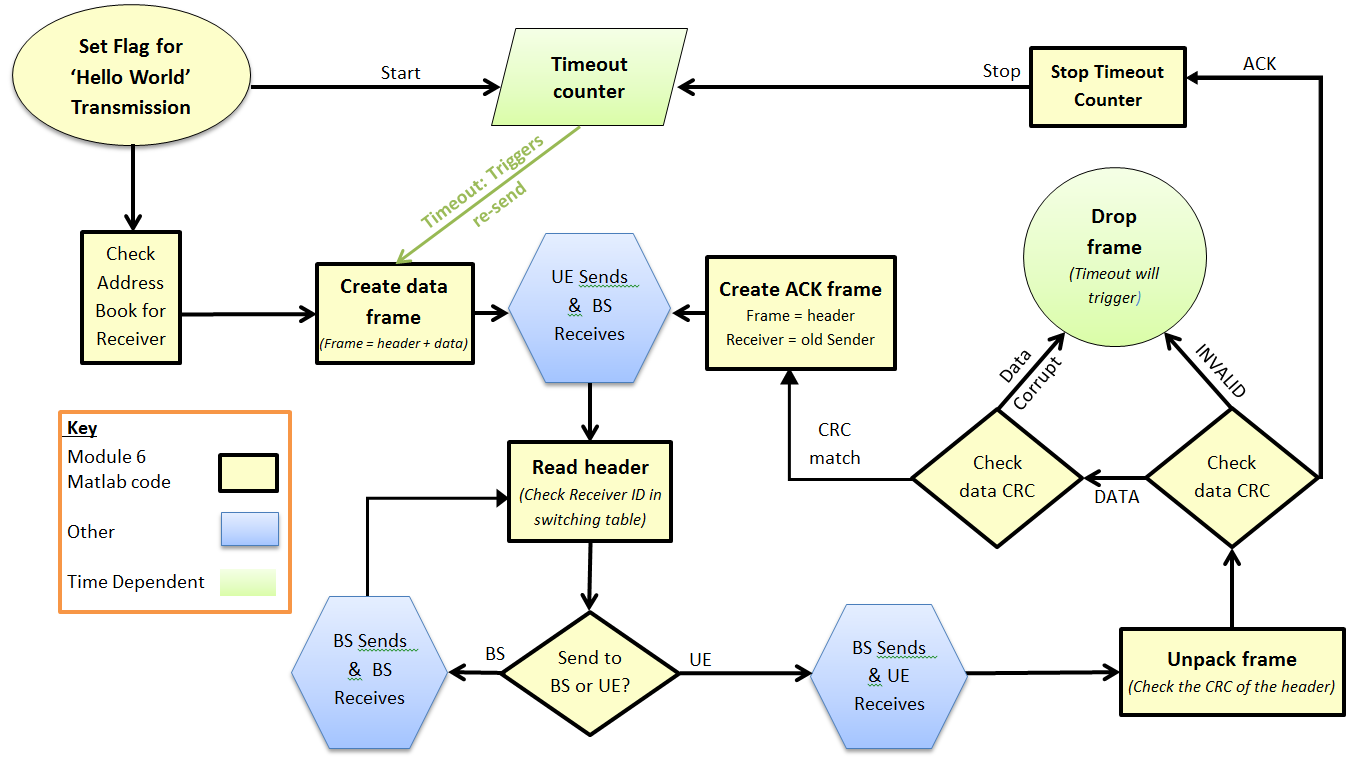
\includegraphics[width=0.8\textwidth]{State_Machine_yellow.PNG}
    \caption{State Machine of the transmission of a package }
    \label{fig:stateMachine}
\end{figure}

\subsection {The ACK response }
The ACK response should only be triggered by the transmission of correct data. We included the CRC of the data field as a section of the data frame so that the CRC can be used to check if the data has changed during any part of it's journey through the network. A data frame which fails the CRC check will have the same result as not receiving any frame at all or of receiving an INVALID frame, no ACK will be sent as seen in Figure \ref{stateMachine}. A correct CRC should trigger the UE to send a ACK with the rec

If there is no ACK received back from the UE that was sent a data frame, then that data frame will eventually have to be resent from the original UE to achieve transmission. The data frame should not be resent before the ACK has an appropriate amount of time to return. Depending on the position of each UE's timeslot in the transmission cycle and whether the UEs are within the same cell, the total time between the the transmission of the data frame and the reception of the ACK will vary greatly. Figure \ref{fig:ACKtimeshort} shows the shortest possible time between transmission and reception. Figure \ref{fig:ACKtimelong} shows the longest, the time increases by a factor of 2. 
\begin{figure}[ht]
    \centering
    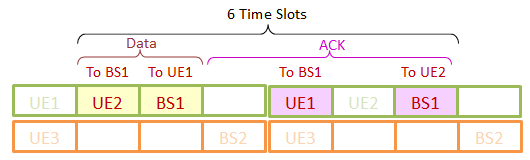
\includegraphics[width=0.8\textwidth]{ACK_timeout_short.PNG}
    \caption{Diagram of the shortest time between a UE transmitting a frame of data and receiving the corresponding ACK}
    \label{fig:ACKtimeshort}
\end{figure}

\begin{figure}[ht]
    \centering
    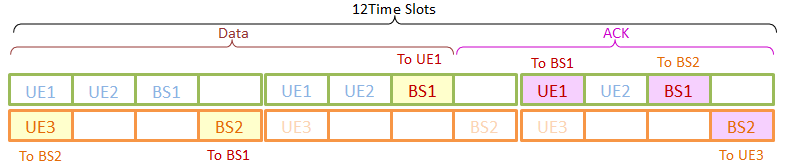
\includegraphics[width=0.8\textwidth]{ACK_timeout_long.PNG}
    \caption{Diagram of the longest time between a UE transmitting a frame of data and receiving the corresponding ACK}
    \label{fig:ACKtimelong}
\end{figure}



% so I am going to be describing the state machine essentially....was going to do this but I might go and write the intro frist to have a beter idea of what is going on.




\section{Frame Types descriptions}
%Renato
We created two frame type baaed on the needs of make a end to end communication.

\begin{description}
  \item[Data Frame] \hfill \\
  It is used to transmit a string message with the limit of 234 bytes. The encode of those bytes is using a ASCII standard. All the bits are order to left most significant bit.
	It is important to guaranteed the decoding of this string in the receiver don’t be machine depend. 
	
  \item[ACK Frame] \hfill \\
  It is the smallest package possible becuase it only have the header information because the data files is not transmitted. It make its transmission time smaller than any data frame. It is reused by Team 4 in their test. 
\end{description}

The frame object was used by other teams so three new types were defined and used by them.
\begin{description}
  \item[REQ Frame] \hfill \\
It is used by Team 4 to request a polling for all devices on the network. It was used by Team 4
	
  \item[Poll Frame] \hfill \\
 It is used by Team 4 to return the polling information of current device to requested polling. 
  \item[Table Frame] \hfill \\
 It is used by Team 5 to return the address table for all devices in the network.

\end{description} 

The frame type was a easy way to change the behavior of the receiving process based on the type.  
%RGB 253 254 202




\chapter{Experimental results}
\label{ch:results}

Put your Experimental results
\section{Testing Frame Construction(FrameObj)}
%Rebecca
% not sure how much of this le will go over...  :/
An easy way of being able to integrate with the other teams seemed to be through the creation of a class, FrameObj, which would not only provide the other modules with a means of creating a frame but a list of properties that could be called for easy debugging. In this object we can also store the values of constants and the ID numbers of devices, statuses, etc.  There are two ways that an instance of the class FrameObj could be constructed,  from the basic requirements of the frame (Frame type, Sender ID number , Receiver ID number, and Data) or from the bits of a frame.

FrameObj was written with a property for almost every field in the frame format. One notable exception is the data field of the frame. The property data is actually a combination of the data field and the CRC for the data. There are some additional properties as well; header and frameArray are not individual fields, instead they combine the fields of the entire header and frame respectively. The property classUse is not intended to be used outside the of the property data, it signifies which of the two ways of class initialization are used so that the data field can operate differently for either as well as for the different frameTypes.
\lstset{caption={Variable Properties of FrameObj},label=propFrameObj} 
\begin{lstlisting} 
    properties
        classUse    %Identifies which configuration was used in this instance of FrameObj
        frameType   %Identifies the type of frame that is being used
        rcvID       %The identification number of the destination receiver
        sndID       %The identification number of the sender.
        data        %The data field (cuts off after more than 234 bytes)
        
    end
    properties (Dependent)
        dataSize    %Indicates the length of the payload in bytes.
        header      %The array of the frame header with hCRC8
        hCRC8       %CRC-8 code verfication of the header field
        dCRC8       %CRC-8 code verfication of the data field
        frameArray  %The frame as an n*1 array
    end
\end{lstlisting}

While writing FrameObj we also wrote the script FrameTest to test the various configurations under which FrameObj might be used. We tried to account for errors, both through using CRCs to protect our bits and by preparing for the rare errors that could happen and not result in an error with the CRC. FrameTest has been re-ordered in sections to best explain the current configuration of FrameObj and not to reflect the code development of FrameObj.

The first section of FrameTest shows the creation of an ACK frame. An ACK is a frame header with the frametype ACKFRAME. In FrameTest it is created from the frame constants: ACKFRAME, UEID1, and UEID2 with a zero entered instead of data.   
\lstset{caption={FrameTest Section 1: ACK},label=FrameTest1} 
\begin{lstlisting}
% create ACK
ACKtype = FrameObj(FrameObj.ACKFRAME, FrameObj.IDUE1, FrameObj.IDUE2, 0);
\end{lstlisting}

These constant properties correspond to the numbers 255, 101, and 102. Instead of just passing frameType=255 through the FrameObj (as we do with device ID numbers) we use a switch statement to compare the frameType input field to the six frameTypes used in FrameObj. The frameType is the most important property of our frame, it is the first part checked every time a frame is received. If a number is used that is not associated with a frameType it will result in a frame that is INVALID.
\lstset{caption={Function defining the frameType property of FrameObj},label=frameType} 
\begin{lstlisting} 
%frameType
        function obj = set.frameType(obj,inputframeType)
            %Using the switch statement in this way ensures that a
            %supported data type is used
            switch inputframeType
                case FrameObj.DATAFRAME     %DATA
                    obj.frameType = uint8(inputframeType);
                case FrameObj.ACKFRAME      %ACK
                    obj.frameType = uint8(inputframeType);
                case FrameObj.POLLFRAME     %POLL
                    obj.frameType = uint8(inputframeType);
                case FrameObj.REQFRAME      %REQ
                    obj.frameType = uint8(inputframeType);
                case FrameObj.TABLEFRAME    %TABLE
                    obj.frameType = uint8(inputframeType);
                case FrameObj.INVALID       %INVALID
                    obj.frameType = uint8(inputframeType);
                otherwise             % also INVALID
                    obj.frameType = uint8(FrameObj.INVALID);
            end
        end
\end{lstlisting}

Many of the other FrameObj properties depend on frameType. For instance ACK has no data CRC, as it has no data. For an FrameObj with frameType ACKFRAME, calling the property dCRC8 would result in an error, halting the program. Similarly, calling dCRC8 will result in an error if an unspecified frameType is used. This aids with frame creation. When an undefined frameType is used, errors will be triggered for each property that depends on frameType until that functionality is added. This way we can be sure that we are not using functionality assumed from other frameTypes. 
\lstset{caption={Function defining the dCRC8 property of FrameObj},label=dCRC8} 
\begin{lstlisting} 
%dCRC8
        %frameType dependent
        function value = get.dCRC8(obj)
            switch obj.frameType
                case FrameObj.DATAFRAME     %DATA
                    %The last byte of obj.data is the CRC. It is seperated
                    %from the data here
                    value = obj.data(end-8:end,1);
                case FrameObj.ACKFRAME      %ACK
                    error('This is an ACK, it has no data therefor no CRC')
                    %If there is no data there should be no check
										....
								otherwise
                    error('Not a supported frame type for dCRC8')
                    % If this error occurs while using a legitimate frame
                    % type please add an addiional case statement for that
                    % frame type.
\end{lstlisting}

No matter what type of valid frame is defined in FrameObj it will always have the same header format and length. The display messages in the command window shown in \ref{fig:FrameTest1} confirm that there are 5 bytes of information in this ACK frame and the dataSize is hard-coded to 0. 

The INVALID frameType is an important part of protecting the class FrameObj from error filled data especially when creating a FrameObj from transceived bits. Critical errors which will cause Matlab errors should result in an INVALID frame. In Section 2 of FrameTest we created three errors that resulted in INVALID frames, the output of this section is shown in \ref{fig:FrameTest2}.
\lstset{caption={FrameTest Section 2: INVALID},label=FrameTest2} 
\begin{lstlisting} 
% nonsense frameType
INVALIDtype = FrameObj(20 , FrameObj.IDUE1, FrameObj.IDUE2, 0);

% cut off the number of bits
receivedshort = ACKtype.frameArray(1:39);
shorttype = FrameObj(receivedshort);

% adds 2000 zeros to the end of the bits 'correct'
% change the sender to IDUE3 to cause the CRC to have an error
receivedcbits = [ACKtype.frameArray; zeros(2000, 1)];
receivedcbits(2*8+1:3*8) =de2bi(uint8(FrameObj.IDUE3),8,'left-msb');
wrongcrc = FrameObj(receivedcbits);
\end{lstlisting} 

The first error, INVALIDtype, is the most straight forward, instead of using a legitimate frametype as the first input to FrameObj, we used an invalid number: 20. This input will be passed to frameType where it will not match any of the defined switch cases in the property frameType shown above and will be set to INVALID through 'otherwise'. The output is shown in \ref{fig:FrameTest2}.  This is the only way to create an INVALID frame by using 4 input fields of FrameObj. 

The next two types of errors that result in INVALID frames are checked for in the FrameObj constructor when the input is in bits. The first of these errors stems from the minimum size of a frame and therefore from the minimum acceptable length of the n*1 input. The array used in FrameObj, receivedshort,  must be at least 40 bits long to represent a valid frame. By defaulting all shorter inputs to INVALID we can be certain that we will not be indexing outside of the dimensions of the input. \ref{fig:FrameTest2} shows that when the input has a length of only 39 bits the resulting frameType will be INVALID. 
\lstset{caption={Single bit array input constructor of FrameObj},label=FrameObj1} 
\begin{lstlisting} 
%Constructor, FrameObj with 1 array of bits
            elseif nargin == 1
                bitwise = inputType;
                 
                %size check
                [size_in, ~] = size(bitwise);
                if (size_in >= 40)
                    % hCRC check
                    hDetect = comm.CRCDetector([8 7 6 4 2 0]);
                    % detects if there is an error in the CRC of the header
                    [~, err] = step(hDetect, bitwise(1:5*8,1));
                    if (err ==0)
																						.....
                    else
                        % the crc does not match and the header is junk
                        obj.frameType = FrameObj.INVALID;
                    end
                else
                    % the data we recdived is not long enough to check the
                    % header crc
                    obj.frameType = FrameObj.INVALID ;     
                end
            else %incorrect number of inputs
                error('That is not a valid number of inputs')
            end
\end{lstlisting} 

The code from the FrameObj constructor above shows the source of the last error that will result in an INVALID frame. After checking for the minimum size of the input, the constructor will check the CRC of the header. In FrameTest we guarantee that the header will cause a CRC error by replacing one UEID number with another in the bit array. An error with the header CRC is not critical for the FrameObj construction but it is important for the functionality of the frame format in the network.

The data field of the frame format is the most complicated property to implement in FrameObj. Not only does it change dramatically with frameType but the way it functions changes with the way that FrameObj is used, with either 1 or 4 inputs. For an ACKFRAME frameType the data property must be initialized as a value or there will be an error but data should not be used. For a DATAFRAME frameType, data must either take in a string or an array of bits. Other frameTypes will have different requirements which means that very little processing can be done in the constructor of the FrameObj, the bulk of data must be defined in the property function. 

Section 3 of TestFrame tests whether the same values for each of the FrameObj properties will be returned. 





\begin{figure}[p]
    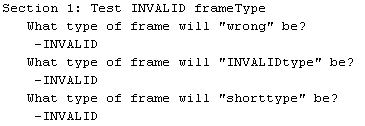
\includegraphics[width=0.5\textwidth, left]{FrameTest1.PNG}
    \caption{Command window output of FrameTest Section 1 showing ACK frame attributes }
    \label{fig:FrameTest1}
\end{figure}

\begin{figure}[p]
    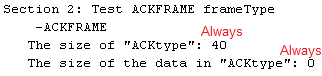
\includegraphics[width=0.55\textwidth, left]{FrameTest2.PNG}
    \caption{Command window output of FrameTest Section 2 showing that all three very wrong frames are INVALID }
    \label{fig:FrameTest2}
\end{figure}

\begin{figure}[p]
    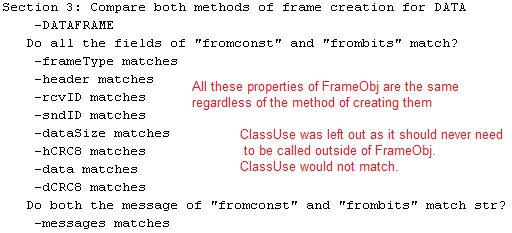
\includegraphics[width=0.77\textwidth, left]{FrameTest3.PNG}
    \caption{Command window output of FrameTest Section 3 showing an instances of FrameObj being created from both types of inputs }
    \label{fig:FrameTest3}
\end{figure}

\begin{figure}[p]
    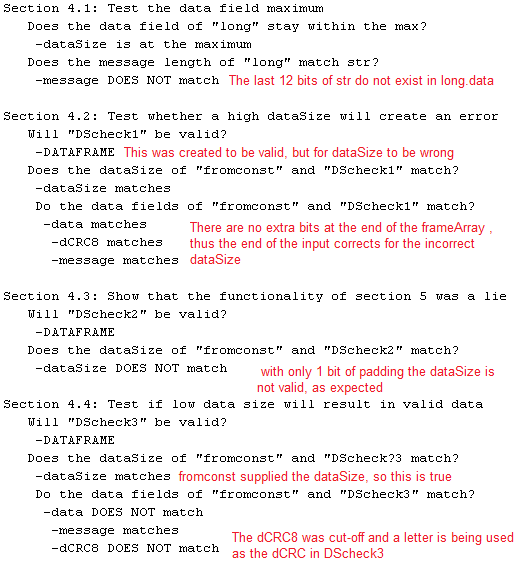
\includegraphics[width=0.77\textwidth, left]{FrameTest4.PNG}
    \caption{Command window output of FrameTest Section 4 showing dataSize limits  }
    \label{fig:FrameTest4}
\end{figure}


\section{End-to-End Local Machine Testing }
%Renato
The test of the implementation of the end to end communication.
Based on proposal of final design project \cite{cdproj}, there
are six case to be tested in the end to end communication
\begin{enumerate}
  \item Extra-cellular communications between UEs
  \begin{enumerate}
    \item US1 $\rightarrow$ BS1 $\rightarrow$ BS2 $\rightarrow$ US3
    \item US3 $\rightarrow$ BS2 $\rightarrow$ BS1 $\rightarrow$ US1
		\item US2 $\rightarrow$ BS1 $\rightarrow$ BS2 $\rightarrow$ US3
		\item US3 $\rightarrow$ BS2 $\rightarrow$ BS1 $\rightarrow$ US2
  \end{enumerate}
  \item Intra-cellular communications between UEs
	  \begin{enumerate}
    \item US1 $\rightarrow$ BS1 $\rightarrow$ US2
    \item US2 $\rightarrow$ BS1 $\rightarrow$ US1
	\end{enumerate}
\end{enumerate}

The figure \ref{fig:endendDiagram} show how the whole MATLAB code is organized to test all the cased described in this section.
The send and received part maps each path of information lie UE 1 to BS1 as a channel . It more logical representation that to a physical channel to the end
to end implementation in the final integration.
The routing used was just a siwtch case based on picture of proposed network in \cite{cdproj}.
The send and received is a recursive function that call it self based with parameters changed for the routing.
One examples is shown in listing \ref{sendReceiveExample} show how inside a channel based on direction how it will resend the message or exit the the function based on the destination.
\lstset{caption={Code examples how to verify the CRC and create the ACK message back to sender},label=sendReceiveExample}
\lstinputlisting{code/sendReceiveExample.M}

The listing \ref{crcVerification} is a examples how the receveive UE in the figure \ref{fig:endendDiagram} verify the CRC and create the new frame to send back.
It procedure is important because it need to be done in the integration with other team that need to use the frameObj.     

\lstset{caption={Code examples how to verify the CRC and create the ACK message back to sender},label=crcVerification}
\lstinputlisting{code/crcVerification.M}



\begin{figure}[ht]
    \centering
    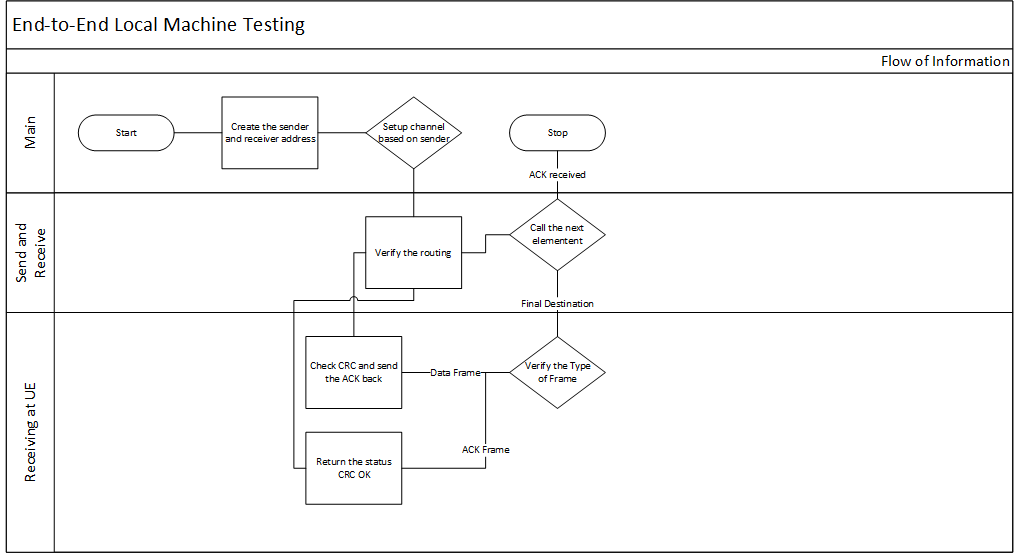
\includegraphics[width=0.8\textwidth]{flowEndtoEnd.PNG}
    \caption{Diagram of the flow of information to test the end to end in Matlab for the team 6 proposed protocol}
    \label{fig:endendDiagram}
\end{figure} 

\section{Transmitting and receiving over the air}
%Renato
The frame object need to be tested over the air to check if it behaves as expected in our simulation. 
It was tested using two different physical layer. 
\subsection{Using lab2 physical layer}

The first test was using a very straight forward approach. We just replaced the 'hello world' message in the Lab 2 
simulating model to add the frame object with a message 'Hi', so it can send a frame near the original size.
The code to create frame is shown in \ref{transLab02}. It is used as input of simulation in diagram of figure \ref{fig:trasmitter_lab02}

\lstset{caption={Code to create the transmitter package to used in Lab 02 physical layer},label=transLab02}
\lstinputlisting{code/crcVerification.M}
\begin{figure}[ht]
    \centering
    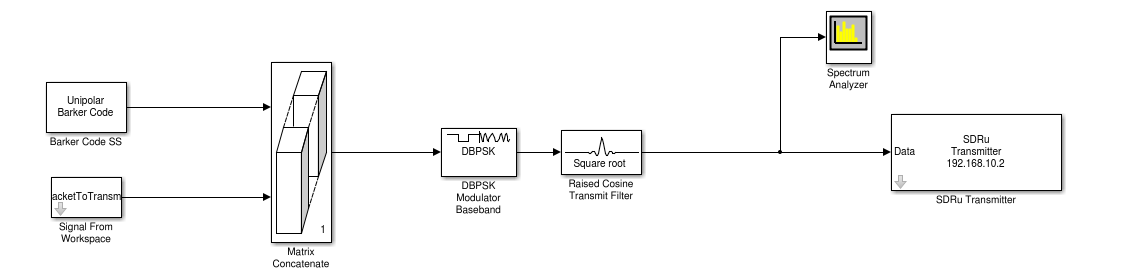
\includegraphics[width=0.8\textwidth]{trasmitter_lab02.PNG}
    \caption{Simulink diagram of the transmitter of the laboratory two physical layer modified to received a input FrameObj wit the message 'Hi' }
    \label{fig:trasmitter_lab02}
\end{figure}

\begin{table}[ht]
	\centering
		\begin{tabular}{| c | c | }
		\hline                       
		Frame Type UE & Number Received\\
		\hline
			ACK & 2\\
			DATA & 102\\
			corrupt DATA & 2\\
			INVALID & 3466\\
			other & 0\\
		\hline
		\end{tabular}
	\caption{Table of frames received with poor transmission quality and a small hamming distance between frame types}
	\label{tab:2ACK}
\end{table}

\begin{table}[ht]
	\centering
		\begin{tabular}{| c | c | }
		\hline                       
		Frame Type & Number Received\\
		\hline
			ACK & 0\\
			DATA & 165\\
			corrupt DATA & 4\\
			INVALID & 3559\\
			other & 0\\
		\hline
		\end{tabular}
	\caption{Table of frames received with poor transmission quality and a larger hamming distance between frame types}
	\label{tab:0ACK}
\end{table}
\subsection{Using Team 4 physical layer}




\chapter{Conclusions}
\label{ch:conclusions}
Put your conlusion here.


%This is the end of my paper.

%%%%%%%%%%%%%%%%%%%%%%%%%%%%%%%% THE FINISH %%%%%%%%%%%%%%%%%%%%%%%%%%%%%%%

%\appendix

% BIBLIOGRAPHY STUFF...
%\nocite{*}
%bibliography stuff

%SEE HERE for BIBTEX styles: http://www.cs.stir.ac.uk/~kjt/software/latex/showbst.html

\bibliographystyle{amsplain}
%\bibliographystyle{plain}

\bibliography{mybib}

%exemple to use the matlab source code
%\lstset{caption={FrameObj Source Code},label=FrameObjSrc}
%\lstinputlisting{code/FrameObj.M}
\appendix 


\chapter{Design Proposal}
\label{ch:proposal}


\includepdf[pages={-}]{ECE4305ProjectProposal6.pdf}



\chapter{Source Code}
\label{ch:code}

%exemple to use the matlab source code
\lstset{caption={FrameObj Source Code},label=FrameObjSrc}
\lstinputlisting{code/FrameObj.M}

\lstset{caption={FrameTest Source Code},label=FrameTestSrc}
\lstinputlisting{FrameTest.M}

\lstset{caption={Receiver code to use the Team 4 physical layer. The explanation of how it works is in section \ref{team4_results} of this resport},label=ReceiverTeam4Code}
\lstinputlisting{code/FrameObj.M}

\end{document}


%useful links:
%latex VS pdflatex : http://www.andy-roberts.net/misc/latex/pdftutorial.html
%basic intro to latex: http://www.andy-roberts.net/misc/latex/latextutorial1.html
%collection of latex links: http://www.andy-roberts.net/misc/index.html
%collection of math symbols: http://www.comp.leeds.ac.uk/andyr/misc/latex/tutorial9/symbols.pdf
%latex matrix examples: http://www.physicsforums.com/showthread.php?t=146358

%lgrind binary for Macintosh:
%https://netfiles.uiuc.edu/galanaki/www/Hints.html
% (place lgrindef in same directory as *.tex, place lgrind in /usr/local/bin

